\documentclass[preprint,11pt]{elsarticle}

\usepackage[utf8]{inputenc}
\usepackage[T1]{fontenc}
\usepackage{lmodern}
\usepackage{amsmath,amssymb,amsthm,mathtools}
\usepackage{graphicx}
\usepackage{booktabs}
\usepackage[shortlabels]{enumitem}
\usepackage{xcolor}
\usepackage[hidelinks]{hyperref}
\usepackage[capitalise,noabbrev]{cleveref}
\usepackage{microtype}
\usepackage{url}

\newtheorem{theorem}{Theorem}[section]
\newtheorem{lemma}[theorem]{Lemma}
\newtheorem{proposition}[theorem]{Proposition}
\newtheorem{corollary}[theorem]{Corollary}
\theoremstyle{definition}
\newtheorem{definition}[theorem]{Definition}
\theoremstyle{remark}
\newtheorem{remark}[theorem]{Remark}

\journal{Theoretical Computer Science}

\begin{document}

\begin{frontmatter}

\title{Towards five-state minimal-time firing squads:\\
a pumping lemma, a speed-$1/3$ barrier, and certified bounds}

\author{Anonymous}
\address{Affiliation withheld for review}

\begin{abstract}
Whether the firing squad synchronization problem admits a minimal-time
solution with five states has been open since Mazoyer's six-state solution
of 1987. We develop general tools for minimal-time solutions and apply them
to this question. First, all lines are encoded by one half-line diagram and
one reflected triangle per length, and each triangle is a function of two
anti-diagonals of the half-line. Second, we prove a pumping lemma: in every
minimal-time solution the inputs of the reflected triangles of any two
lengths $n<n'$ differ on a cone of about $n/2$ cells. The lemma constrains
the half-line alone and implies a speed-$1/3$ barrier: the non-periodic part
of the half-line always reaches the line $i=t/3$. Third, we give a
propositional encoding of the bounded problem together with these
constraints, validate it against Mazoyer's solution extracted from a Coq
formalization, and obtain a certified (LRAT-checked) re-proof of the
nonexistence of four-state minimal-time solutions in under a minute.
Finally, we report an extensive search for five-state solutions.

\end{abstract}

\begin{keyword}
firing squad synchronization problem \sep cellular automata \sep state
complexity \sep minimal time \sep SAT solving \sep proof certificates
\end{keyword}

\end{frontmatter}

%% ---------------------------------------------------------------------
\section{Introduction}\label{sec:intro}

The firing squad synchronization problem (FSSP), posed by Myhill in 1957
and popularised by Moore~\cite{Moore64}, asks for a finite automaton that,
placed in every cell of a line of arbitrary length $n$ and started with all
cells quiescent except a \emph{general} at one end, drives all cells into a
common \emph{firing} state for the first time at the same instant. Goto
\cite{Goto62} and Waksman \cite{Waksman66} showed that this is possible in
time $2n-2$, which is optimal \cite{Moore64}. Since then the minimum number
of states of a \emph{minimal-time} solution has been a benchmark question
in cellular automata theory \cite{Mazoyer86,Umeo09}: Waksman used $16$
states, Balzer $8$ \cite{Balzer67}, Gerken $7$ \cite{Gerken87} and Mazoyer
$6$ \cite{Mazoyer87}. On the other side, Balzer \cite{Balzer67} reported,
and Sanders \cite{Sanders94} confirmed with a corrected exhaustive search,
that no $4$-state minimal-time solution exists. Whether five states suffice
has remained open since Mazoyer's construction; it is regarded as the
central open question on state complexity of the FSSP
\cite{Umeo09,Correa17}. Many six-state minimal-time solutions are known
today \cite{Clergue18,NguyenMaignan20}, and five-state solutions are known
for restricted families of lengths or for non-minimal time
\cite{UmeoYanagihara07,Yunes08,UmeoKamikawaYunes09}, but no five-state
minimal-time solution has been found, nor has its existence been refuted.

\paragraph{This paper.}
We develop tools that apply to minimal-time solutions with any number of
states and use them to attack the five-state question.
\begin{enumerate}[label=(\roman*)]
\item \emph{Agreement and reflection.} We make explicit the elementary but
  useful fact that the line of length $n$ coincides with the half-line below
  the anti-diagonal $t+i=2n-2$, so that all lines are encoded by a single
  half-line diagram $C_\infty$ plus one ``reflected triangle'' $R_n$ per
  length, and that $R_n$ is a function of two anti-diagonals of $C_\infty$
  only (\cref{sec:prelim,sec:pumping}).
\item \emph{A pumping lemma.} We prove that in every minimal-time solution
  the input words of the reflected triangles are pairwise distinct on a cone
  of length about $n/2$ (\cref{lem:pumping}). This is a constraint on the
  half-line alone, valid for \emph{all} pairs of lengths, and it implies a
  \emph{speed-$1/3$ barrier} (\cref{thm:third}): the periodic regime behind
  the front can never overtake a signal of speed $1/3$ emitted by the
  general. This gives an a priori explanation of the speed-$1/3$ signal
  present in all classical constructions.
\item \emph{A certified SAT framework.} We encode ``there is a $k$-state rule
  that synchronizes a given set of lengths in minimal time, together with
  the pumping constraints and further consequences'' into propositional
  logic (\cref{sec:encoding}). The encoding re-derives the non-existence of
  four-state minimal-time solutions in less than a minute on a laptop core,
  and it is validated against Mazoyer's six-state solution extracted from
  the Coq formalization of Duprat \cite{Duprat97}.
\item \emph{Five states.} We report the outcome of the search for five-state
  solutions (\cref{sec:experiments}).
\end{enumerate}

\paragraph{Related work.}
Surveys of the FSSP are \cite{Mazoyer86,Umeo09}. Beyond Balzer and Sanders,
lower bounds on the number of states are known for variants: no three-state
solution and no four-state symmetric minimal-time solution exist for rings
\cite{BerthiaumeEtAl04}; for further restricted classes see
\cite{Correa17}. Computer searches have been used to find new
solutions \cite{Clergue18} and to generate families of solutions by local
simulations \cite{NguyenMaignan20}. SAT solvers have been applied to many
extremal problems in combinatorics with certified unsatisfiability proofs
\cite{HeuleKullmannMarek16,Heule18}; to our knowledge this is the first
SAT-based treatment of the FSSP state-complexity question.

%% ---------------------------------------------------------------------
\section{Preliminaries}\label{sec:prelim}

\subsection{The problem}

Let $S$ be a finite set of \emph{states} containing three distinguished
elements: the \emph{quiescent} state $\mathsf L$, the \emph{general}
$\mathsf G$ and the \emph{firing} state $\mathsf F$; these are pairwise
distinct. We write $W:=S\setminus\{\mathsf F\}$ for the set of
\emph{working} states and use a symbol $\ast\notin S$ for the border.
A \emph{rule} is a map
\[
\delta:\;(W\cup\{\ast\})\times W\times(W\cup\{\ast\})\;\longrightarrow\;S
\]
satisfying the quiescence conditions
\begin{equation}\label{eq:quiescence}
\delta(\mathsf L,\mathsf L,\mathsf L)=\delta(\mathsf L,\mathsf L,\ast)=\mathsf L .
\end{equation}
(Transitions out of $\mathsf F$ and transitions whose neighbourhood contains
$\mathsf F$ play no role below and are left unspecified; we do \emph{not}
require $\delta(\ast,\mathsf L,\mathsf L)=\mathsf L$, which only strengthens
the non-existence statements.)

For $n\ge 1$ the \emph{line of length $n$} is the space-time diagram
$C_n:\mathbb N\times\{1,\dots,n\}\to S$ defined by
$C_n(0,1)=\mathsf G$, $C_n(0,i)=\mathsf L$ for $2\le i\le n$, and
\[
C_n(t+1,i)=\delta\bigl(C_n(t,i-1),\,C_n(t,i),\,C_n(t,i+1)\bigr),
\]
with the convention $C_n(t,0)=C_n(t,n+1)=\ast$; the diagram is only
considered up to the first time at which some cell is in state $\mathsf F$.
The rule \emph{synchronizes the line of length $n$ at time $T$} if
$C_n(T,i)=\mathsf F$ for all $1\le i\le n$ and $C_n(t,i)\neq\mathsf F$ for all
$t<T$ and all~$i$.

It is classical \cite{Moore64,Waksman66,Balzer67} that no rule synchronizes a
line of length $n\ge2$ before time $2n-2$ (see also \cref{lem:return}
below). A \emph{minimal-time solution} is a rule that synchronizes the line
of length $n$ at time exactly $2n-2$ for every $n\ge2$. (For $n=1$ one
usually asks $\delta(\ast,\mathsf G,\ast)=\mathsf F$; this transition is
used by no other line and is irrelevant here.) A \emph{$k$-state solution} is
one with $|S|=k$.

More generally, for a set $\mathcal N\subseteq\{2,3,\dots\}$ of lengths, a
rule is \emph{$\mathcal N$-minimal} if it synchronizes the line of length $n$
at time $2n-2$ for every $n\in\mathcal N$. Clearly a minimal-time solution
is $\mathcal N$-minimal for every $\mathcal N$; all our non-existence
arguments exhibit a finite family of necessary conditions that no $5$-state
rule satisfies.

\subsection{The half-line and the agreement lemma}

Let $C_\infty:\mathbb N\times\{1,2,\dots\}\to S$ be the diagram of the
half-line: $C_\infty(0,1)=\mathsf G$, $C_\infty(0,i)=\mathsf L$ for $i\ge2$,
and the same recurrence with a border on the left only.

\begin{lemma}[light cone]\label{lem:lightcone}
For every rule, every $n$ and every $(t,i)$ with $t<i-1$ we have
$C_n(t,i)=C_\infty(t,i)=\mathsf L$.
\end{lemma}

\begin{proof}
By induction on $t$. For $t=0$ this is the initial condition. Let $t\ge1$
and $t<i-1$. The three cells $(t-1,i-1),(t-1,i),(t-1,i+1)$ satisfy
$t-1<(i-1)-1$, hence are in state $\mathsf L$ by induction, except that the
right neighbour of cell $n$ of $C_n$ is the border. By \eqref{eq:quiescence}
the new state is $\mathsf L$ in both cases.
\end{proof}

\begin{lemma}[agreement]\label{lem:agree}
For every rule and every $n\ge 2$: $C_n(t,i)=C_\infty(t,i)$ whenever
$1\le i\le n$ and $t+i\le 2n-2$.
\end{lemma}

\begin{proof}
Induction on $t$; the case $t=0$ is clear. Let $t\ge1$ and $t+i\le 2n-2$.
If $i=n$ then $t\le n-2<i-1$ and both sides equal $\mathsf L$ by
\cref{lem:lightcone}. If $i<n$, the three neighbours $(t-1,j)$,
$j\in\{i-1,i,i+1\}$, satisfy $(t-1)+j\le t+i\le 2n-2$ and $j\le n$, so they
agree by induction (for $j=0$ both are the border). Hence the new states
agree.
\end{proof}

Thus the right border of the line of length $n$ is first ``felt'' at the
cell $(n-1,n)$, and its influence is confined to the \emph{reflected
triangle}
\[
R_n:=\{(t,i):\ 1\le i\le n,\ t+i\ge 2n-1,\ t\le 2n-2\}.
\]

\begin{lemma}[return chain]\label{lem:return}
Let $\delta$ synchronize the lines of lengths $n$ and $n+1$ at times $2n-2$
and $2n$ respectively. Then
\[
C_n(2n-1-i,\,i)\;\neq\;C_\infty(2n-1-i,\,i)\qquad(1\le i\le n).
\]
In particular the \emph{front} $s_i:=C_\infty(i-1,i)$ satisfies
$s_{n-1}\neq\mathsf L$, and $\delta(s_{n-1},\mathsf L,\ast)\neq
\delta(s_{n-1},\mathsf L,\mathsf L)$.
\end{lemma}

\begin{proof}
For $i=1$: $C_n(2n-2,1)=\mathsf F$ while, by \cref{lem:agree} applied to
the line of length $n+1$ (note $(2n-2)+1\le 2(n+1)-2$),
$C_\infty(2n-2,1)=C_{n+1}(2n-2,1)\neq\mathsf F$ because $2n-2<2n$.
Suppose the claim holds for some $i<n$. The cell $(2n-1-i,i)$ is computed
from the cells $(2n-2-i,j)$, $j=i-1,i,i+1$, whose coordinate sums are
$2n-3$, $2n-2$ and $2n-1$. By \cref{lem:agree} the first two are the same
in $C_n$ and $C_\infty$ (for $i=1$ the left neighbour is the border in both
diagrams). Since the results differ, the right neighbours differ:
$C_n(2n-2-i,i+1)\ne C_\infty(2n-2-i,i+1)$, which is the claim for $i+1$.
For $i=n$ we get $C_n(n-1,n)=\delta(s_{n-1},\mathsf L,\ast)\neq
C_\infty(n-1,n)=\delta(s_{n-1},\mathsf L,\mathsf L)=s_n$, which is impossible
if $s_{n-1}=\mathsf L$ by \eqref{eq:quiescence}.
\end{proof}

Applying \cref{lem:return} to all $n$ shows that in a minimal-time
solution every cell $i$ leaves $\mathsf L$ exactly at time $i-1$ (the front
moves at speed one) and, since $C_\infty(t,i)=C_{n}(t,i)$ for $n$ large,
\begin{equation}\label{eq:neverfire}
C_\infty(t,i)\neq\mathsf F\qquad\text{for all }t\ge0,\ i\ge1 .
\end{equation}

%% ---------------------------------------------------------------------
\section{Reflected triangles and a pumping lemma}\label{sec:pumping}

\subsection{Relative coordinates}

Fix $n\ge2$. For a cell $(t,i)$ of the line of length $n$ put
$\tau:=t-(n-1)$ (time elapsed since the front reached the right end) and
$\kappa:=n-i$ (distance to the right end). Then
\[
R_n=\{(\tau,\kappa):\ 0\le\kappa\le\tau\le n-1\},
\]
the right border sits at $\kappa=-1$ and the left border at $\kappa=n$.
A cell $(\tau,\kappa)\in R_n$ is computed from
$(\tau-1,\kappa+1),(\tau-1,\kappa),(\tau-1,\kappa-1)$; each of these is
either in $R_n$, or a border, or satisfies $\tau'-\kappa'\in\{-1,-2\}$,
i.e.\ lies on one of the anti-diagonals $t+i=2n-2$, $t+i=2n-3$, where
$C_n$ coincides with $C_\infty$ by \cref{lem:agree}. We call
\[
J_n(\kappa):=\bigl(C_\infty(n-3+\kappa,\,n-\kappa),\;C_\infty(n-2+\kappa,\,n-\kappa)\bigr),
\qquad 0\le\kappa\le n-1,
\]
the \emph{input word} of $R_n$; its two components are the \emph{lower}
($t+i=2n-3$) and \emph{upper} ($t+i=2n-2$) input cells.

\begin{lemma}[determinacy]\label{lem:determinacy}
There is a single partial map $\Psi$, depending on $\delta$ only, such that
for every $n\ge2$ and every $(\tau,\kappa)\in R_n$,
$C_n\bigl(n-1+\tau,\,n-\kappa\bigr)$ is obtained by evaluating $\Psi$ at
$(\tau,\kappa)$ on the input word $J_n$ with borders at $\kappa=-1$ and
$\kappa=n$. In particular the value only depends on the input cells and
borders in the backward dependency cone of $(\tau,\kappa)$.
\end{lemma}

\begin{proof}
The recurrence in relative coordinates does not mention $n$; only the
position of the left border does.
\end{proof}

For $(\tau,\kappa)\in R_n$ let $\mathrm{cone}_n(\tau,\kappa)$ be the set of
input cells (pairs $(\kappa',\text{lower/upper})$) reached from
$(\tau,\kappa)$ by repeatedly passing to the three predecessors, stopping at
input cells and borders; say that the cone is \emph{right-anchored} if it
does not reach the left border $\kappa'=n$.

\begin{lemma}\label{lem:cone}
For $n\ge4$ the cone of the right end at the firing time,
$\mathrm{cone}_n(n-1,0)$, is right-anchored and consists of the upper input
cell at $\kappa'=0$, both input cells at $1\le\kappa'\le\lfloor n/2\rfloor$,
and, when $n$ is odd, the lower input cell at $\kappa'=(n+1)/2$.
\end{lemma}

\begin{proof}
A predecessor step changes $\tau$ by $-1$ and $\kappa$ by at most one, and
input cells satisfy $\tau'=\kappa'-1$ or $\kappa'-2$. Starting from
$(n-1,0)$, a path that reaches an input cell at position $\kappa'$ after $s$
steps satisfies $\kappa'\le s$ and $n-1-s=\kappa'-1$ or $\kappa'-2$; hence
$2\kappa'\le n+1$ (upper cells: $2\kappa'\le n$). Conversely every such cell
is reached by the path that first moves left $\kappa'$ times and then stays
put (the intermediate cells lie in $R_n$). The largest $\kappa'$ reached is
$\lceil n/2\rceil\le n-1$ for $n\ge 4$, so the left border is never reached;
the right border only contributes the constant symbol~$\ast$. (The same set
is also computed mechanically in the accompanying code, file
\texttt{pumping.py}.)
\end{proof}

\begin{lemma}[pumping]\label{lem:pumping}
Let $\delta$ be a minimal-time solution and $4\le n<n'$. Then $J_n$ and
$J_{n'}$ differ on $\mathrm{cone}_n(n-1,0)$.
\end{lemma}

\begin{proof}
Suppose they agree there. By \cref{lem:determinacy,lem:cone} the relative
cell $(n-1,0)$ of $R_{n'}$ (which belongs to $R_{n'}$ since $n-1\le n'-1$,
and whose cone is the same set of input positions, far from the left border
$\kappa=n'>n$) has the same value as the relative cell $(n-1,0)$ of $R_n$,
namely $C_n(2n-2,n)=\mathsf F$. Thus $C_{n'}(n'+n-2,n')=\mathsf F$ although
$n'+n-2<2n'-2$, contradicting minimality for $n'$.
\end{proof}

The point of \cref{lem:pumping} is that it constrains the \emph{half-line
diagram only}: no reflected triangle has to be computed. It is the source of
the constraint family $\mathrm{PUMP}(n,n')$ used in \cref{sec:encoding}. As a
sanity check, we verified mechanically that Mazoyer's six-state solution
satisfies $\mathrm{PUMP}(n,n')$ for all $4\le n<n'\le120$.

\subsection{Consequence: a speed-$1/3$ barrier}

Write the half-line diagram in the frame of the front:
$\Phi_t(j):=C_\infty(t,\,t+1-j)$ for $0\le j\le t$ (the cell at
\emph{depth}~$j$ behind the front at time~$t$). By the recurrence,
\begin{equation}\label{eq:comoving}
\Phi_{t+1}(j)=\delta\bigl(\Phi_t(j),\,\Phi_t(j-1),\,\Phi_t(j-2)\bigr)
\qquad(0\le j\le t),
\end{equation}
with $\Phi_t(-1)=\Phi_t(-2)=\mathsf L$: in this frame the half-line is a
\emph{one-sided} automaton in which information only travels to larger
depths, at most two depths per step. In particular every depth-row
$t\mapsto\Phi_t(j)$ is eventually periodic.
In these coordinates
$J_n(\kappa)=\bigl(\Phi_{n-3+\kappa}(2\kappa-2),\ \Phi_{n-2+\kappa}(2\kappa-1)\bigr)$.

\begin{theorem}[speed-$1/3$ barrier]\label{thm:third}
Let $\delta$ be a minimal-time solution and suppose that the depth-rows have
a common eventual period: there are $P\ge1$ and thresholds $T(j)$ with
$\Phi_{t+P}(j)=\Phi_t(j)$ for all $t\ge T(j)$. Then for every $n\ge4$ there
is a depth $j\le n$ with $T(j)>n+\tfrac{j}{2}-\tfrac52$. Consequently
$\limsup_{j\to\infty}T(j)/j\ge 3/2$; in the original coordinates, the
periodic regime behind the front cannot overtake the line $i=t/3$.
\end{theorem}

\begin{proof}
If every input cell of $\mathrm{cone}_n(n-1,0)$ is read in the periodic
regime of its row, i.e.\ $n-3+\kappa\ge T(2\kappa-2)$ and
$n-2+\kappa\ge T(2\kappa-1)$ for all cone positions, then
$J_{n+P}=J_n$ on the cone, contradicting \cref{lem:pumping}. The cone
positions satisfy $\kappa\le\lceil n/2\rceil$, so the violated inequality
concerns a depth $j\in\{2\kappa-2,2\kappa-1\}$, $j\le n$, with
$T(j)>n-3+\kappa\ge n+\frac{j}{2}-\frac52$. If $T(j)\le\alpha j+\beta$ for
all~$j$ with $\alpha<3/2$, then for $n$ large and all $j\le n$ we have
$\alpha j+\beta\le n+\frac j2-\frac52$ (as $(\alpha-\frac12)j\le(\alpha-\frac12)n
<n-\beta-\frac52$), a contradiction. A cell of depth $j$ at time $T(j)$ has
position $T(j)+1-j$, whence the geometric statement.
\end{proof}

\Cref{thm:third} explains a posteriori the ubiquity of the speed-$1/3$
signal emitted by the general in the classical constructions
\cite{Waksman66,Balzer67,Mazoyer87}: its crossing with the anti-diagonal
$t+i=2n-2$ is exactly the far end of $\mathrm{cone}_n(n-1,0)$. It also
explains the failure mode of the ``lucky'' partial solutions found by the
solvers, whose half-line diagrams become periodic behind the front at
speed larger than $1/3$ (see \cref{sec:experiments}).

%% ---------------------------------------------------------------------
\section{Propositional encoding}\label{sec:encoding}

Fix $k$ (the number of states), write $W=\{\mathsf L,\mathsf G,a_1,\dots,a_{k-3}\}$
and let $\mathcal N$ be a finite set of lengths. We build a CNF formula
$\mathrm{MT}_k(\mathcal N;M,N')$ that is satisfiable whenever a $k$-state
minimal-time solution exists. All constraint families below are either the
definition of $\mathcal N$-minimality or consequences of
\cref{lem:agree,lem:return,lem:determinacy,lem:pumping} and
\eqref{eq:neverfire}; none relies on unproved assumptions about the shape of
solutions.

\paragraph{Variables}
For every neighbourhood $e=(x,y,z)\in(W\cup\{\ast\})\times W\times(W\cup\{\ast\})$
other than $(\ast,y,\ast)$, one-hot variables $T_{e,d}$, $d\in S$, encode
$\delta(e)=d$; the two quiescence transitions \eqref{eq:quiescence} are fixed
by unit clauses. For every cell whose state is not a constant, one-hot
variables $X_{c,s}$, $s\in W$, encode its state (all cells whose state is
used before the firing time are in $W$).

\paragraph{Transition clauses}
For a cell $c$ with neighbours $c_1,c_2,c_3$ (cells, constants $\mathsf L,
\mathsf G$, or the border) and for all $(x,y,z)$ in the respective domains
and $d\in W$ we add
\begin{align*}
&\neg X_{c_1,x}\vee\neg X_{c_2,y}\vee\neg X_{c_3,z}\vee\neg T_{(x,y,z),d}\vee X_{c,d},\\
&\neg X_{c_1,x}\vee\neg X_{c_2,y}\vee\neg X_{c_3,z}\vee\neg T_{(x,y,z),\mathsf F}
\end{align*}
(the second clause forbids firing). For a cell that must fire we add instead
$\neg X_{c_1,x}\vee\neg X_{c_2,y}\vee\neg X_{c_3,z}\vee T_{(x,y,z),\mathsf F}$.
Literals of constant neighbours are omitted.

\paragraph{Half-line} The cells $(t,i)$ of $C_\infty$ with $1\le i\le t+1$
and $t+i\le M$ receive variables and transition clauses; cells with
$i>t+1$ are the constant $\mathsf L$ (\cref{lem:lightcone}). Every such cell
is forbidden to fire, by \eqref{eq:neverfire}.

\paragraph{Lines} For every $n\in\mathcal N$ (with $2n-2\le M$) the cells of
$R_n$ with $t\le 2n-3$ receive variables; their neighbours outside $R_n$ are
the corresponding half-line cells (\cref{lem:agree}). All of them are
forbidden to fire and the $n$ cells at time $2n-2$ are required to fire.

\paragraph{Return chains} For $n\in\mathcal N$ with $2n-1\le M$ we add the
implied constraints $C_n(2n-1-i,i)\ne C_\infty(2n-1-i,i)$ of
\cref{lem:return} (their derivation only uses \eqref{eq:neverfire} at the
cell $(2n-2,1)$, which is part of the encoding).

\paragraph{Pumping} For all $4\le n<n'\le N'$ (with $2N'-2\le M$) we add one
clause stating that $J_n$ and $J_{n'}$ differ on $\mathrm{cone}_n(n-1,0)$,
introducing an auxiliary ``difference'' variable for every pair of
non-constant input cells (\cref{lem:pumping}).

\paragraph{Determinacy links} For $n<n'$ in $\mathcal N$ and $p\ge0$ an
auxiliary variable $E_{n,n'}(p)$ is made equivalent to ``$J_n$ and $J_{n'}$
coincide on the positions $0,\dots,p$''. For every relative cell
$(\tau,\kappa)$ of $R_n$ whose dependency cone is right-anchored and contained
in the positions $0,\dots,p$ we add
$E_{n,n'}(p)\Rightarrow\bigl(R_n(\tau,\kappa)=R_{n'}(\tau,\kappa)\bigr)$,
and, for the firing cells $\tau=n-1$, the clause $\neg E_{n,n'}(p)$
(\cref{lem:determinacy,lem:pumping}). These clauses are implied by the
others but allow the solver to transfer information between lines.

\paragraph{Symmetry breaking} Permuting the auxiliary states maps
solutions to solutions. We require that, in the time-major enumeration of
the encoded half-line cells, the first occurrence of $a_{j}$ precedes the
first occurrence of $a_{j+1}$; every solution can be renamed to satisfy
this. For $k=5$ this halves the search space.

\paragraph{Soundness checks}
Besides the proofs above, every constraint family was tested against an
independent ground truth: Mazoyer's six-state solution, extracted
mechanically from Duprat's Coq formalization \cite{Duprat97}, satisfies
the formula $\mathrm{MT}_6(\mathcal N;78,40)$ for
$\mathcal N=\{3,\dots,12\}$ with return chains, pumping and links (the
formalization does not cover $n=2$), and it satisfies
$\mathrm{MT}_6(\{3,\dots,14\};26)$ with symmetry breaking under exactly one
of the $3!$ renamings of its auxiliary states, as it must. Conversely, every
model found by the solvers was decoded and re-simulated by an independent
brute-force checker (\texttt{fsspcheck.c}), which confirmed minimal-time
synchronization for all encoded lengths.

%% ---------------------------------------------------------------------
\section{Experiments}\label{sec:experiments}

\paragraph{Setup.} Formulas are generated by \texttt{gencnf.py} and solved
with Kissat \cite{Kissat20} (default configuration unless stated) or, for
incremental runs, with CaDiCaL~1.9.5 through PySAT \cite{PySAT18}. Every
model is decoded into a rule table and re-simulated by the independent
checker \texttt{fsspcheck.c}, which reports the first length (if any) that
is not synchronized in minimal time. All timings are single-core wall-clock
times on a cloud virtual CPU.

\subsection{Calibration: four and six states}

\begin{table}[t]
\centering\small
\begin{tabular}{@{}p{0.47\textwidth}p{0.33\textwidth}r@{}}
\toprule
instance & result & time\\
\midrule
$\mathrm{MT}_4(\{2,\dots,8\};14)$ & SAT (27 partial rules) & $1.7$\,s\\
$\mathrm{MT}_4(\{2,\dots,9\};16)$ & UNSAT & $24.7$\,s\\
$\mathrm{MT}_4(\{2,\dots,10\};18)$ & UNSAT & $26.8$\,s\\
$\mathrm{MT}_4(\{2,\dots,7\};78,40)$ + links & SAT (model fails at $n=8$) & $27.5$\,s\\
$\mathrm{MT}_4(\{2,\dots,8\};78)$, lazy & UNSAT & $46.6$\,s\\
\midrule
Mazoyer's rule and $\mathrm{MT}_6(\{3,\dots,12\};78,40)$ + links & SAT (as required) & ---\\
$\mathrm{MT}_6(\{2,\dots,12\};78,40)$ & SAT, model fails at $n=13$ & $534$\,s\\
\bottomrule
\end{tabular}
\caption{Calibration. $\mathrm{MT}_k(\mathcal N;M,N')$: lengths $\mathcal N$,
half-line up to anti-diagonal $M$, pumping pairs up to $N'$ (omitted when not
used).}\label{tab:calibration}
\end{table}

For four states our encoding reproduces the theorem of Balzer and Sanders
within half a minute (\cref{tab:calibration}): the formula for the lengths
$2,\dots,9$ is unsatisfiable, whereas $27$ partial rules (counted on the
transitions they actually use, by an independent depth-first enumeration
exploring $1.09\cdot10^8$ nodes) synchronize all lengths $2,\dots,8$.
Extending the half-line to anti-diagonal $78$ already rules out lengths
$2,\dots,8$. Note that we do not assume $\delta(\ast,\mathsf L,\mathsf L)=
\mathsf L$, so this is a slight strengthening of the four-state result.

For six states the solver finds models as well, but, instructively, the
first model found for the lengths $2,\dots,12$ is not a solution: it fails at
$n=13$ although millions of genuine six-state solutions exist
\cite{NguyenMaignan20}. This ``lucky rule'' phenomenon dominates the
five-state landscape.

\subsection{Five states: the landscape of lucky rules}

\Cref{tab:five} summarizes the five-state instances solved so far. Two kinds
of lucky rules appear. Rules of the first kind have a \emph{periodic}
half-line behind the front (\cref{fig:diagrams}(b)); they satisfy a long
line such as $n=20$ by accident but violate the pumping constraints
massively (155 violated pairs $4\le n<n'\le40$ for the rule shown). Rules of
the second kind have a chaotic half-line that eventually fires. Once the
half-line is extended and the pumping constraints are added, the solver is
forced to produce half-lines with a genuine slow boundary: in every model we
inspected, a region delimited by a line of slope $1/3$ appears
(\cref{fig:diagrams}(c)), exactly as predicted by \cref{thm:third}. The
reflected triangles of these rules, however, synchronize only the lengths
that were encoded.

\begin{table}[t]
\centering\small
\begin{tabular}{@{}lll@{}}
\toprule
instance ($k=5$) & result & time\\
\midrule
$\mathrm{MT}_5(\{2,\dots,10\};18)$ & SAT, fails at $n=11$ & $10.8$\,s\\
$\mathrm{MT}_5(\{2,\dots,12\};22)$ & SAT, fails at $n=13$ & $\approx 20$\,min\\
$\mathrm{MT}_5(\{2,\dots,9,16\};30)$ & SAT, fails at $n=10$ & $23.6$\,s\\
$\mathrm{MT}_5(\{2,\dots,9,20\};38)$ & SAT, fails at $n=10$ & $82.4$\,s\\
$\mathrm{MT}_5(\{2,\dots,8\};78,40)$ & SAT, fails at $n=9$ & $68.7$\,s\\
$\mathrm{MT}_5(\{2,\dots,10\};78,40)$ & SAT, fails at $n=11$ & $755.6$\,s\\
$\mathrm{MT}_5(\{2,\dots,11\};78)$, lazy & SAT, fails at $n=12$ & $773.9$\,s\\
\bottomrule
\end{tabular}
\caption{Five-state instances (notation as in \cref{tab:calibration}).}
\label{tab:five}
\end{table}

\begin{figure}[t]
\centering
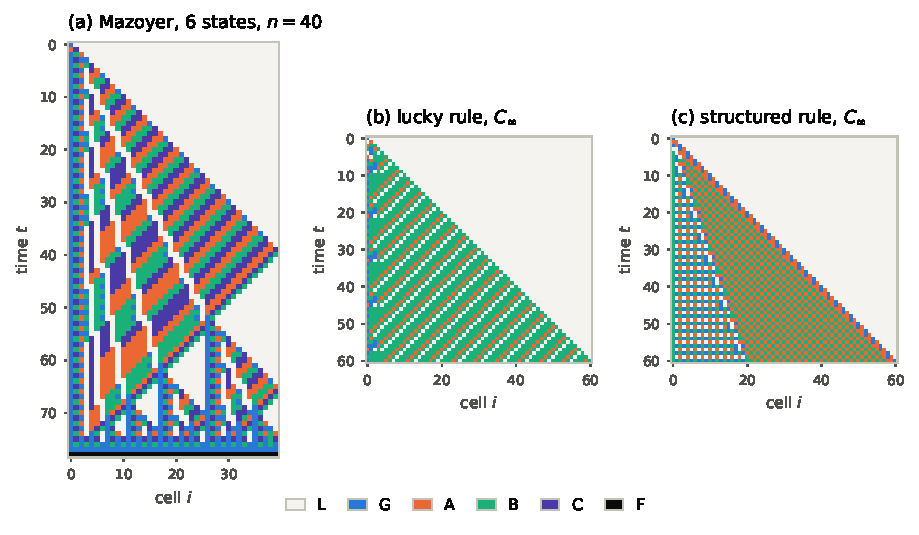
\includegraphics[width=\textwidth]{fig_diagrams.pdf}
\caption{Space-time diagrams (time downwards). (a) Mazoyer's six-state
solution on $n=40$ cells; the last row is the firing row. (b) Half-line of a
five-state rule that synchronizes the lengths $2,\dots,9$ and $20$ but
violates the pumping lemma: its background is periodic. (c) Half-line of a
five-state rule found under the pumping constraints: the boundary between
the checkered region and the diagonal background has slope $1/3$.}
\label{fig:diagrams}
\end{figure}

%% ---------------------------------------------------------------------
\section{Discussion}\label{sec:discussion}

\paragraph{What the pumping lemma buys}
\Cref{lem:pumping} turns an infinite family of requirements on the
reflected triangles into constraints on the half-line diagram only. It is
satisfied by Mazoyer's solution, as it must be, and it eliminates, at
negligible cost, the whole class of rules whose half-line becomes periodic
behind the front too early. \Cref{thm:third} shows that the constraint has a
transparent geometric meaning: in every minimal-time solution the
non-periodic part of the half-line reaches the line $i=t/3$. For Mazoyer's
solution every depth-row is $3$-periodic from time $2j+1$ or $2j+2$, i.e.\
the periodic zone behind the front is bounded by a signal of speed $1/2$,
comfortably within the bound.

\paragraph{Why lucky rules are hard to kill}
Small sets of necessary conditions are typically met by rules that are not
solutions; the question is how many lengths are needed before all such rules
disappear (if no solution exists, some finite set of lengths suffices, since
there are finitely many rules). For four states the answer is $9$ (or $8$ with a long
half-line). For five states the rule space is larger by roughly $38$
orders of magnitude ($5^{94}$ versus $4^{45}$ transition tables), and our
experiments show partial rules for all lengths up to at least $12$, and for
any single additional length we tried. Under the pumping constraints the
surviving rules are no longer random: their half-lines exhibit a speed-$1/3$
boundary, and the remaining freedom lies in the reflected triangles.

\paragraph{The mirrored construction}
The cone of \cref{lem:cone} ends where the anti-diagonal $t+i=2n-2$ meets
the line $i=t/3$. By \cref{lem:determinacy}, the part of $R_n$ whose cone lies
in the periodic zone behind the front is the same for all large $n$ of a
given residue class, and the information that makes the right end fire
exactly at time $2n-2$ enters $R_n$ near that crossing and travels to the
right end at maximal speed. Heuristically, the right half of every
reflected triangle therefore has to behave like a \emph{mirrored}
minimal-time synchronization, started by the reflection and running on the
background left behind the front instead of on quiescent cells. A
five-state solution would have to realize both constructions---the direct
one on the quiescent background and the mirrored one on the front's
background---with the same four working states. We regard this tension as
the structural reason why five states are hard; turning it into a theorem
(for instance a mirrored version of \cref{thm:third}, for which the missing
ingredient is a border at the far end of the mirrored problem) is the most
promising route to a conceptual proof.

\paragraph{Open problems}
\begin{enumerate}[label=(\arabic*)]
\item Does a five-state minimal-time solution exist? By
  \cref{thm:frontier}, a negative answer along the lines of \cref{thm:four}
  requires lines of length at least $13$.
\item Is there a necessary condition, in the spirit of \cref{lem:pumping},
  that constrains the reflected triangles themselves and not only the
  half-line?
\item What is the smallest $N$ such that some five-state rule is
  $\{2,\dots,N\}$-minimal but no five-state rule is
  $\{2,\dots,N+1\}$-minimal, if such an $N$ exists?
\end{enumerate}


\section*{Data availability}
All programs, CNF generators, solver logs, rule tables and proof certificates
are available in the accompanying repository (directory \texttt{fssp5/}).

\bibliographystyle{elsarticle-num}
\bibliography{refs}

%% ---------------------------------------------------------------------
\appendix

\section{The rule of \cref{thm:frontier}}\label{app:delta12}

\begin{table}[p]
\centering\small
\begin{tabular}{@{}cc|ccccc@{}}
\toprule
left & centre & \multicolumn{5}{c}{right neighbour}\\
 & & $\ast$ & $\mathsf{L}$ & $\mathsf{G}$ & $\mathsf{A}$ & $\mathsf{B}$\\
\midrule
$\ast$ & $\mathsf{L}$ & -- & $\mathsf{A}$ & $\mathsf{A}$ & $\mathsf{A}$ & $\mathsf{A}$\\
$\mathsf{L}$ & $\mathsf{L}$ & $\mathsf{L}$ & $\mathsf{L}$ & $\mathsf{L}$ & $\mathsf{B}$ & $\mathsf{A}$\\
$\mathsf{G}$ & $\mathsf{L}$ & $\mathsf{A}$ & $\mathsf{G}$ & $\mathsf{G}$ & $\mathsf{L}$ & $\mathsf{A}$\\
$\mathsf{A}$ & $\mathsf{L}$ & $\mathsf{B}$ & $\mathsf{A}$ & $\mathsf{B}$ & $\mathsf{A}$ & $\mathsf{A}$\\
$\mathsf{B}$ & $\mathsf{L}$ & $\mathsf{G}$ & $\mathsf{B}$ & $\mathsf{L}$ & $\mathsf{A}$ & $\mathsf{A}$\\
\midrule
$\ast$ & $\mathsf{G}$ & -- & $\mathsf{A}$ & $\mathsf{A}$ & $\mathsf{A}$ & $\mathsf{A}$\\
$\mathsf{L}$ & $\mathsf{G}$ & $\mathsf{B}$ & $\mathsf{B}$ & $\mathsf{G}$ & $\mathsf{L}$ & $\mathsf{B}$\\
$\mathsf{G}$ & $\mathsf{G}$ & $\mathsf{G}$ & $\mathsf{G}$ & $\mathsf{G}$ & $\mathsf{A}$ & $\mathsf{B}$\\
$\mathsf{A}$ & $\mathsf{G}$ & $\mathsf{A}$ & $\mathsf{L}$ & $\mathsf{A}$ & $\mathsf{A}$ & $\mathsf{G}$\\
$\mathsf{B}$ & $\mathsf{G}$ & $\mathsf{B}$ & $\mathsf{G}$ & $\mathsf{L}$ & $\mathsf{A}$ & $\mathsf{A}$\\
\midrule
$\ast$ & $\mathsf{A}$ & -- & $\mathsf{G}$ & $\mathsf{B}$ & $\mathsf{F}$ & $\mathsf{L}$\\
$\mathsf{L}$ & $\mathsf{A}$ & $\mathsf{A}$ & $\mathsf{L}$ & $\mathsf{A}$ & $\mathsf{A}$ & $\mathsf{B}$\\
$\mathsf{G}$ & $\mathsf{A}$ & $\mathsf{B}$ & $\mathsf{L}$ & $\mathsf{A}$ & $\mathsf{B}$ & $\mathsf{A}$\\
$\mathsf{A}$ & $\mathsf{A}$ & $\mathsf{F}$ & $\mathsf{B}$ & $\mathsf{G}$ & $\mathsf{F}$ & $\mathsf{A}$\\
$\mathsf{B}$ & $\mathsf{A}$ & $\mathsf{A}$ & $\mathsf{B}$ & $\mathsf{A}$ & $\mathsf{G}$ & $\mathsf{A}$\\
\midrule
$\ast$ & $\mathsf{B}$ & -- & $\mathsf{A}$ & $\mathsf{A}$ & $\mathsf{A}$ & $\mathsf{A}$\\
$\mathsf{L}$ & $\mathsf{B}$ & $\mathsf{G}$ & $\mathsf{B}$ & $\mathsf{L}$ & $\mathsf{B}$ & $\mathsf{B}$\\
$\mathsf{G}$ & $\mathsf{B}$ & $\mathsf{A}$ & $\mathsf{A}$ & $\mathsf{B}$ & $\mathsf{B}$ & $\mathsf{G}$\\
$\mathsf{A}$ & $\mathsf{B}$ & $\mathsf{L}$ & $\mathsf{B}$ & $\mathsf{A}$ & $\mathsf{A}$ & $\mathsf{G}$\\
$\mathsf{B}$ & $\mathsf{B}$ & $\mathsf{G}$ & $\mathsf{A}$ & $\mathsf{B}$ & $\mathsf{B}$ & $\mathsf{L}$\\
\bottomrule
\end{tabular}
\caption{The five-state rule $\delta_{12}$ of \cref{thm:frontier}: entry $\delta(\text{left},\text{centre},\text{right})$. The entries $\delta(\mathsf L,\mathsf L,\mathsf L)=\delta(\mathsf L,\mathsf L,\ast)=\mathsf L$ are the quiescence conditions; ``--'' marks the unused neighbourhoods $(\ast,y,\ast)$. Machine-readable copy: \texttt{results/uniformA\_2-12.txt}.}
\label{tab:delta12}
\end{table}


\section{Reproducibility}\label{app:repro}

The directory \texttt{fssp5/} of the accompanying repository contains all
programs, the rule tables and the logs. The main components are:
\begin{description}[style=nextline,leftmargin=1.5em,font=\normalfont]
\item[\texttt{src/fsspcheck.c}] independent brute-force simulator: reads a
  rule table and checks minimal-time synchronization for a range of lengths
  (full simulation of every line, no use of the agreement lemma);
\item[\texttt{src/gencnf.py}] CNF generator for $\mathrm{MT}_k(\mathcal N;M,N')$
  with the options of \cref{sec:encoding} (return chains, pumping, links,
  symmetry breaking) and the restricted classes used in the experiments;
\item[\texttt{src/pumping.py}] computation of the cones of
  \cref{lem:cone} by breadth-first search and direct verification of
  $\mathrm{PUMP}(n,n')$ on a given rule;
\item[\texttt{src/fsspdfs.c}] exhaustive depth-first enumeration of partial
  rules (\cref{tab:four});
\item[\texttt{src/mazoyer\_from\_coq.py}] extraction of Mazoyer's rule from
  the file \texttt{autom.v} of Duprat's Coq development \cite{Duprat97};
\item[\texttt{src/validate\_mazoyer.py}] soundness test of the encoding;
\item[\texttt{src/check\_halfline.py}] direct check that a half-line
  diagram has no firing cell below a given anti-diagonal;
\item[\texttt{src/fixgerm.py}, \texttt{src/knuth.py},
  \texttt{src/benders.py}] the experiments of \cref{sec:five}.
\end{description}

\paragraph{Certificate for \cref{thm:four}}
{\footnotesize
\begin{verbatim}
python3 gencnf.py 4 9 mt4_9.cnf
cadical --lrat --binary=false mt4_9.cnf mt4_9.lrat  # UNSAT
lrat-check mt4_9.cnf mt4_9.lrat                     # VERIFIED
\end{verbatim}}
SHA-256 digests (each on two lines):
{\footnotesize
\begin{verbatim}
mt4_9.cnf           d18d65480e77505193b8f60362badad5
                    e71f8f08505f29befbcd3b2b18cdaabf
mt4_9.lrat          1d511a75ab25587fa4a3476b95ad3f71
                    33c7375ad96661fd22fa598aec6c8092
uniformA_2-12.txt   b62abbcac0653a661cd1bbe344dee9db
                    ba0cddee37448ea16681d436166c3aad
mazoyer6.txt        4b0717ea7319957c1fdcc887fe09c107
                    4cf338e8b849cdd32b4307d0083f417e
\end{verbatim}}

\paragraph{Checking \cref{thm:frontier}}
{\footnotesize
\begin{verbatim}
R=results/uniformA_2-12.txt
fsspcheck $R 2 12              # OK for all 2 <= n <= 12
fsspcheck $R 13 13             # FAIL: a cell fires at time 23
python3 pumping.py $R 40       # 0 violations
python3 check_halfline.py $R 78  # no firing cell, t+i <= 78
\end{verbatim}}
The uniform configuration before firing in (a) is visible with the option
\texttt{-v} of the checker, which prints the diagrams.

\paragraph{Validation against Mazoyer's solution}
{\footnotesize
\begin{verbatim}
python3 mazoyer_from_coq.py autom.v > mazoyer6.txt
fsspcheck mazoyer6.txt 3 3000   # OK for all 3 <= n <= 3000
python3 validate_mazoyer.py 14  # SAT under exactly one renaming
\end{verbatim}}


\end{document}
